\documentclass{article}
\usepackage[utf8]{inputenc}
\usepackage{indentfirst}
\usepackage{graphicx}
\usepackage[nottoc,notlot,notlof]{tocbibind}
 
\begin{document}

\begin{center}
{\large Master 1 - Ingénierie Informatique} \\ [0.5cm]
\vfill
\rule{\linewidth}{0.4mm} \\ [0.4cm]
{\huge \bfseries
Travaux d'Etude et de Recherche\\
- \\
GraphoScan \\ [0.4cm]
Mémoire Intermédiaire \\ [0.4cm]
}
\rule{\linewidth}{0.4mm} \\ [1.5cm]

\begin{minipage}{0.4\textwidth}
\begin{flushleft} \large
Thibault \textsc{Charpignon} \\
Benoît \textsc{Gallet} \\
Emmanuel \textsc{Herrmann} \\
Martin \textsc{Réty}
\end{flushleft}
\end{minipage}

\vfill

\large\emph{Encadré par : }{Matthieu \textsc{Exbrayat}}

\vfill


{\large 6 Février - 13 Mars 2017}

\end{center}

\newpage
 
\tableofcontents

\newpage
 
\section{Résumé du projet}

\subsection{Présentation}

Ce projet de TER prolonge un travail déjà entamé l'année dernière par deux étudiants de Polytech, consistant à enregistrer en vidéo l'écriture d'un calligraphe, pour pouvoir reconstruire un modèle en 3D du mouvement de la plume. Une structure en bois supporte deux caméras, que l'on peut bouger le long de rails puis fixer à l'aide de vis. Le calligraphe écrit sous cette structure et la feuille est éclairée par des spots lumineux. Il faut alors associer l'image des deux caméras, ce qui n'est pas possible nativement avec le logiciel fourni par le fabricant (FlyCapture de PointGrey) pour faire de l'acquisition vidéo en stéréo, puis reconstituer via OpenGL les mouvements de la plume. Ces mouvements ont été sauvegardés grâce à des algorithmes de tracking, travaillant sur les vidéos enregistrées auparavant.



\subsection{But du projet}

Ce projet permettra à terme de réaliser une reconstitution 3D des mouvements du calligraphe. On pourra alors lui faire recopier plusieurs textes, provenant de différents lieux et différentes époques, afin de pouvoir comparer les styles d'écriture, définir s'il existait différentes écoles d'écriture, différents styles, etc. De manière plus générale, le projet pourra servir pour beaucoup d'applications par la suite, car le code final se voudra le plus généraliste possible.

\section{Introduction au domaine}


Le programme en lui-même est entièrement réalisé en C++, et différentes librairies graphiques sont utilisées dans ce projet pour le traitement du flux vidéo, dans le but de faire du tracking sur le résultat, notamment OpenGl et OpenCV. OpenGL est utilisé pour la reconstruction du mouvement de la plume en 3D, tandis qu'OpenCV est plus utilisé pour le traitement de l'image, notamment toutes les opérations faites dessus. De plus, Matlab est utilisé pour effectuées diverses opérations mathématiques sur les images, comme par exemple l'enlèvement de la distorsion. En effet, comme les caméras ont un grand angle, les éléments sur le bord de l'image sont courbés, il faut donc les remettre droit pour pouvoir travailler dessus.

\section{Analyse de l'existant}

\subsection{Fonctionnement de l'application}

Cette section présente le fonctionnement global de l'application, afin de mieux cerner le sujet sur lequel nous avons travaillé. Il faut cependant préciser que ce n'est pas sous cette forme que nous avons reçu le projet, il ne fonctionnait que partiellement, la version présentée ici est la version finale post-TER.

\begin{figure}[!h]
\centering
\includegraphics[scale=0.08]{Modules/Picture/Utilisation.png}
\caption{Ecriture et acquisition}
\label{utilisation}
\end{figure}

Le dispositif montré sur la figure \ref{utilisation} nous permet de capturer les vidéos en direct. Ces deux vidéos sont enregistrées sur ordinateur, pour pouvoir faire de la stéréo : on encode les images en même temps pour avoir exactement les mêmes frames au même moment. On applique ensuite des paramètres d'undistortion pour lisser les bords de l'image. En effet, la caméra ayant un grand angle, l'extérieur de l'image est déformé, ce qui peut apporter des problèmes lors de la reconstruction 3D.

Une fois les deux vidéos récupérées, on peut lancer la reconstruction. La première étape est de retrouver l'écriture sur l'image, pour cela différentes méthodes sont disponibles. On peut par exemple faire du tracking. Après avoir sélectionné une zone d'intérêt grâce à un ROI (Region Of Interest) selector (figure \ref{ROI} ), on essaye de suivre le mouvement. Il suffit d'enregistrer les coordonnées du centre du point pour retrouver le mouvement dessiné (figure \ref{tracking} ).

La seconde technique est celle du HOG (Histogramme de gradient orienté) qui permet de détecter des formes dans une image. Ce qui donne au départ une image comme sur la figure \ref{HOGSale}, et après nettoyage \ref{HOGPropre}.

L'une ou l'autre de ces techniques peuvent être utilisées pour avoir une suite de coordonnées correspondant au dessin de l'écriture. Une fois que ces deux coordonnées sont récupérées, il existe des fonctions dans OpenCV pour faire des points 3D à partir de points 2D. Il faut pour cela récupérer les paramètres extrinsèques (matrices de rotation et vecteurs de translation, pour passer du repère lié à l'espace de travail au repère lié à la caméra) de la caméra.

Une fois que les coordonnées sont récupérées par l'une ou l'autre méthode, une fonction nous permet de rajouter deux points entre chaque coordonnée pour fluidifier la ligne. Ces coordonnées sont ensuite interprétées par OpenGL pour permettre de les afficher dans un repère en trois dimensions (figures \ref{3D1} et \ref{3D2} ).


\begin{figure}[htb]
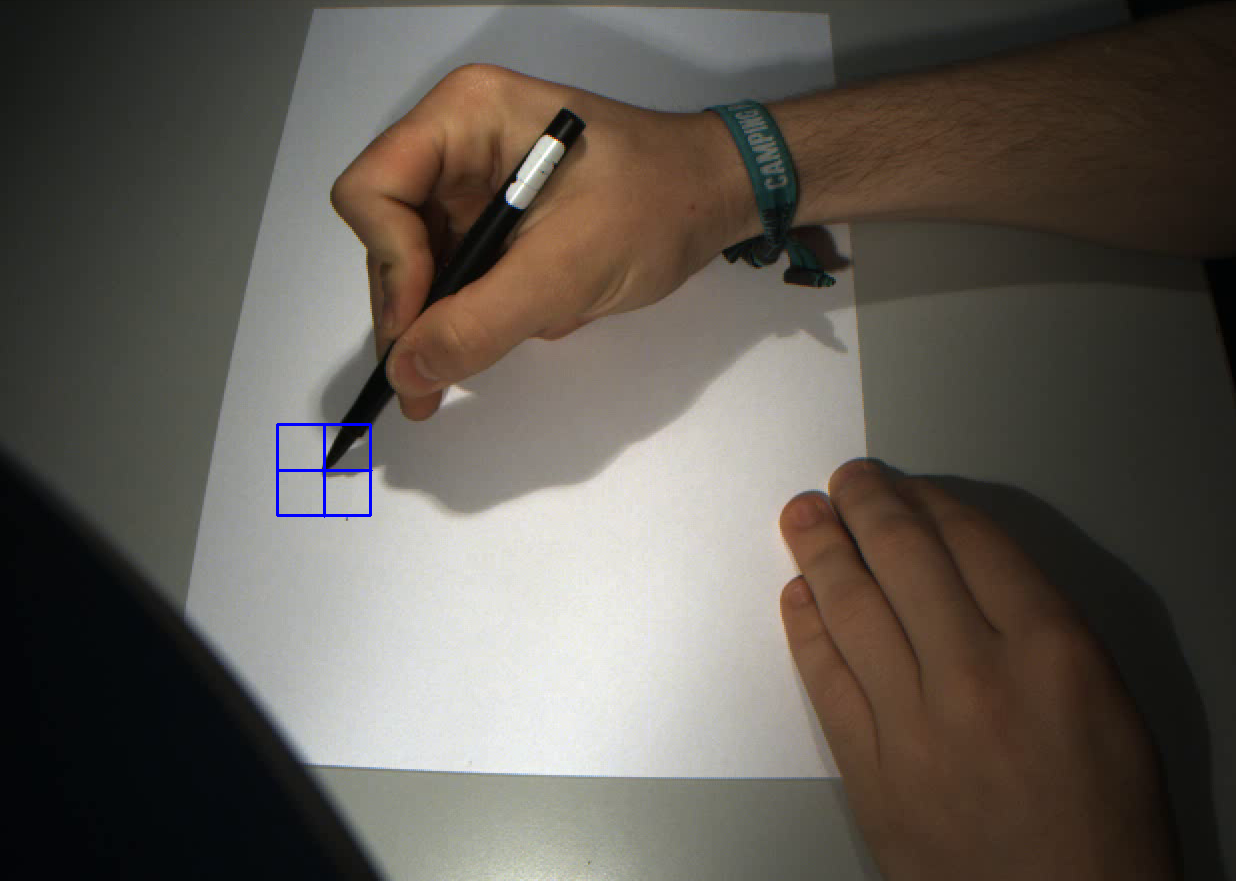
\includegraphics[width=\textwidth]{Modules/Picture/roi}
\caption{ROI selector}
\label{ROI}
\vspace{30px}
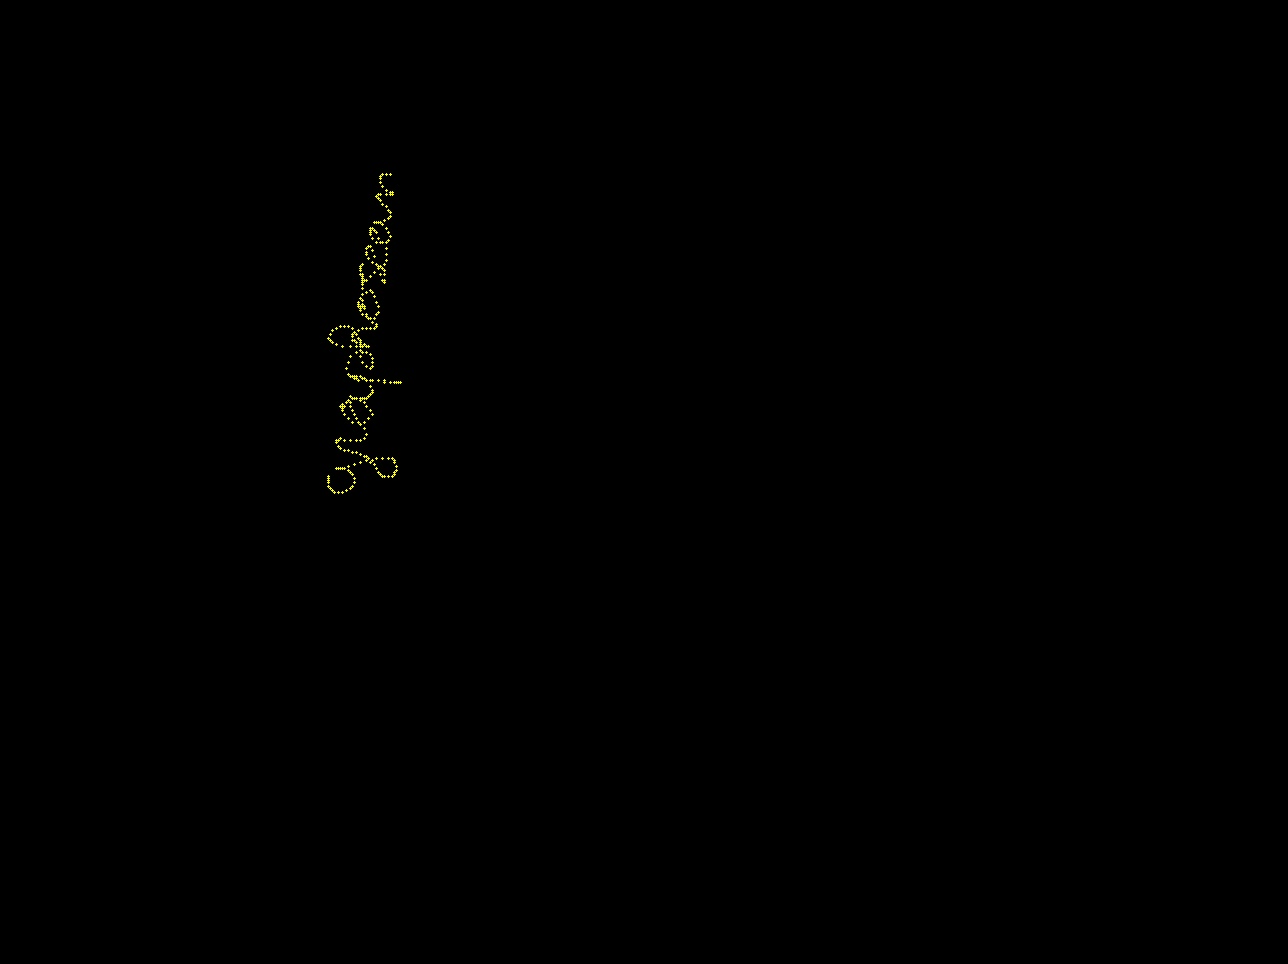
\includegraphics[width=\textwidth]{Modules/Picture/tracking}
\caption{Reconnaissance avec le tracking}
\label{tracking}
\end{figure}

\newpage

\begin{figure}
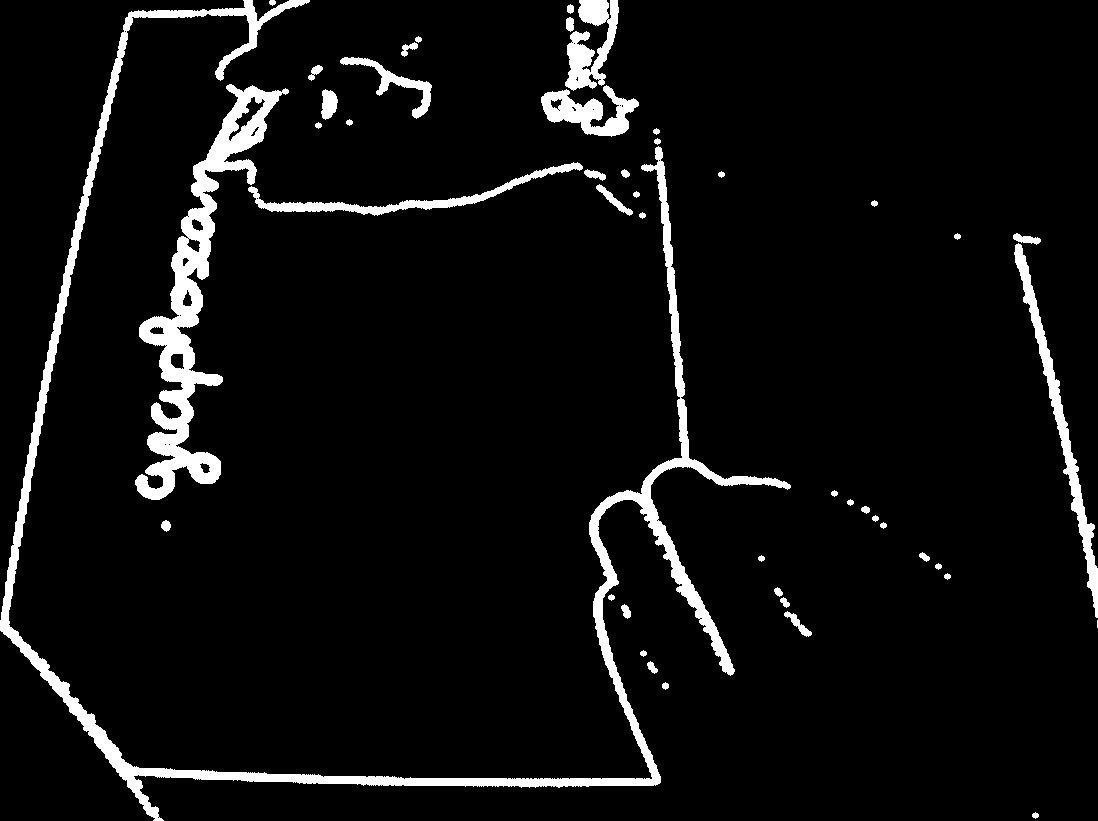
\includegraphics[width=\textwidth]{Modules/Picture/hog}
\caption{HOG brut}
\label{HOGSale}
\vspace{30px}
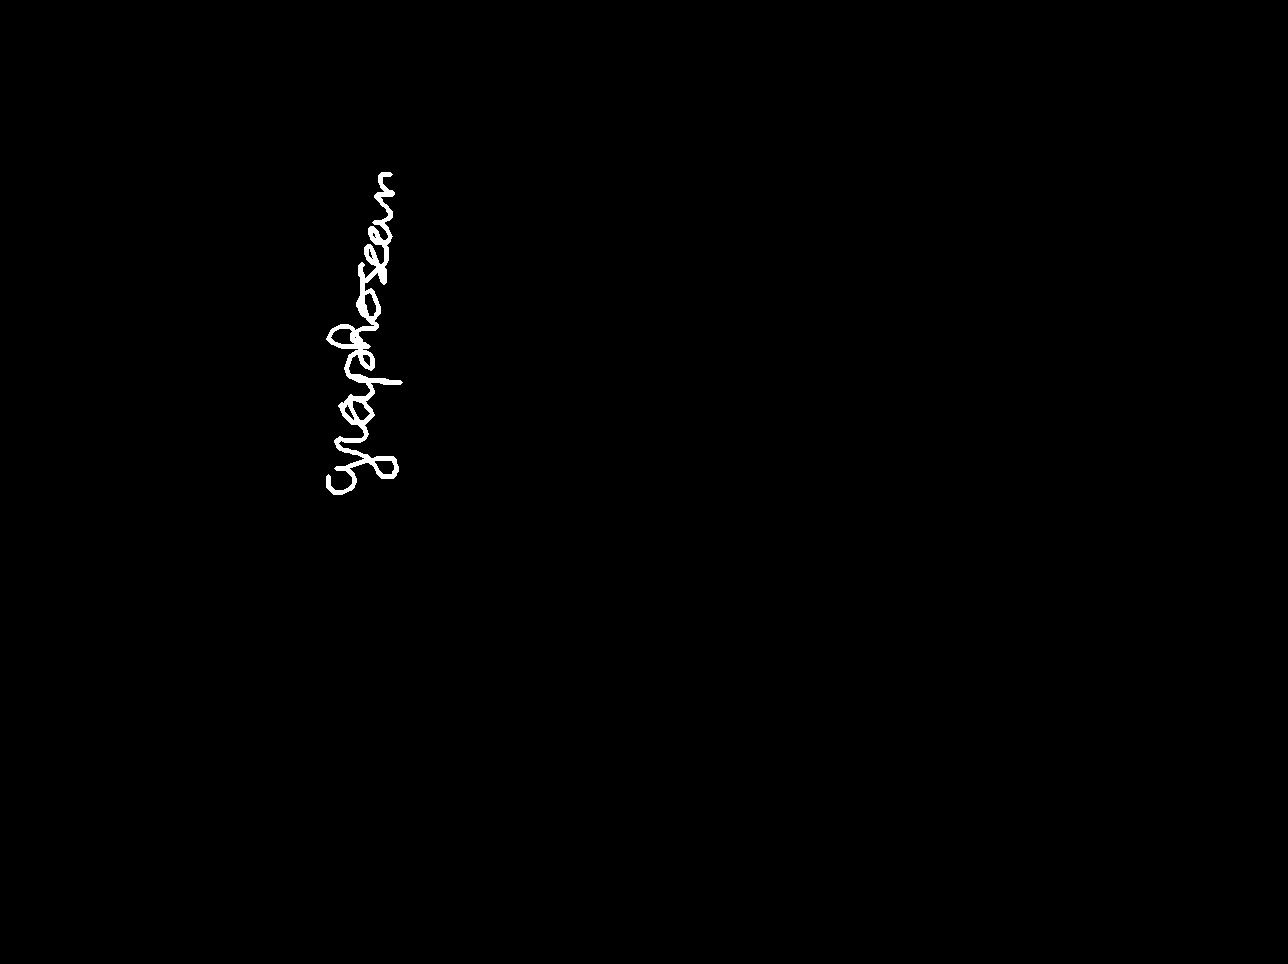
\includegraphics[width=\textwidth]{Modules/Picture/hog_propre}
\caption{HOG nettoyé}
\label{HOGPropre}
\end{figure}

\newpage

\begin{figure}
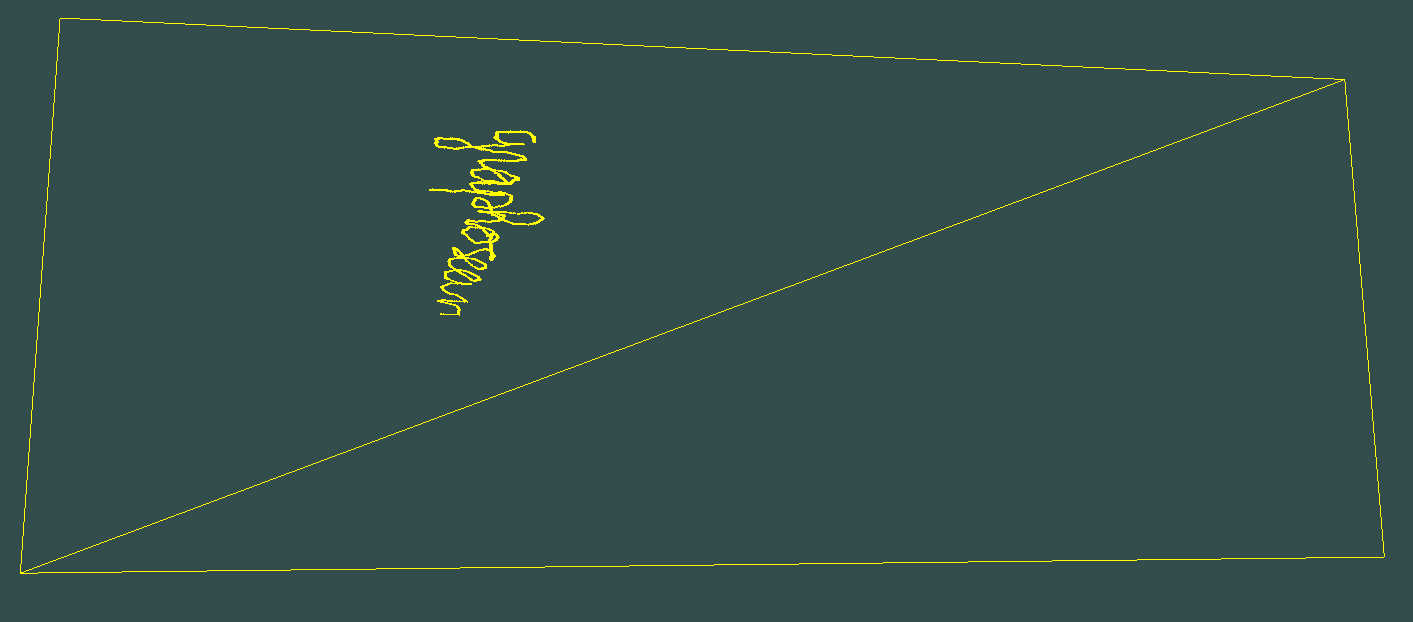
\includegraphics[width=\textwidth]{Modules/Picture/3d_1}
\caption{Image 3D - 1}
\label{3D1}
\vspace{30px}
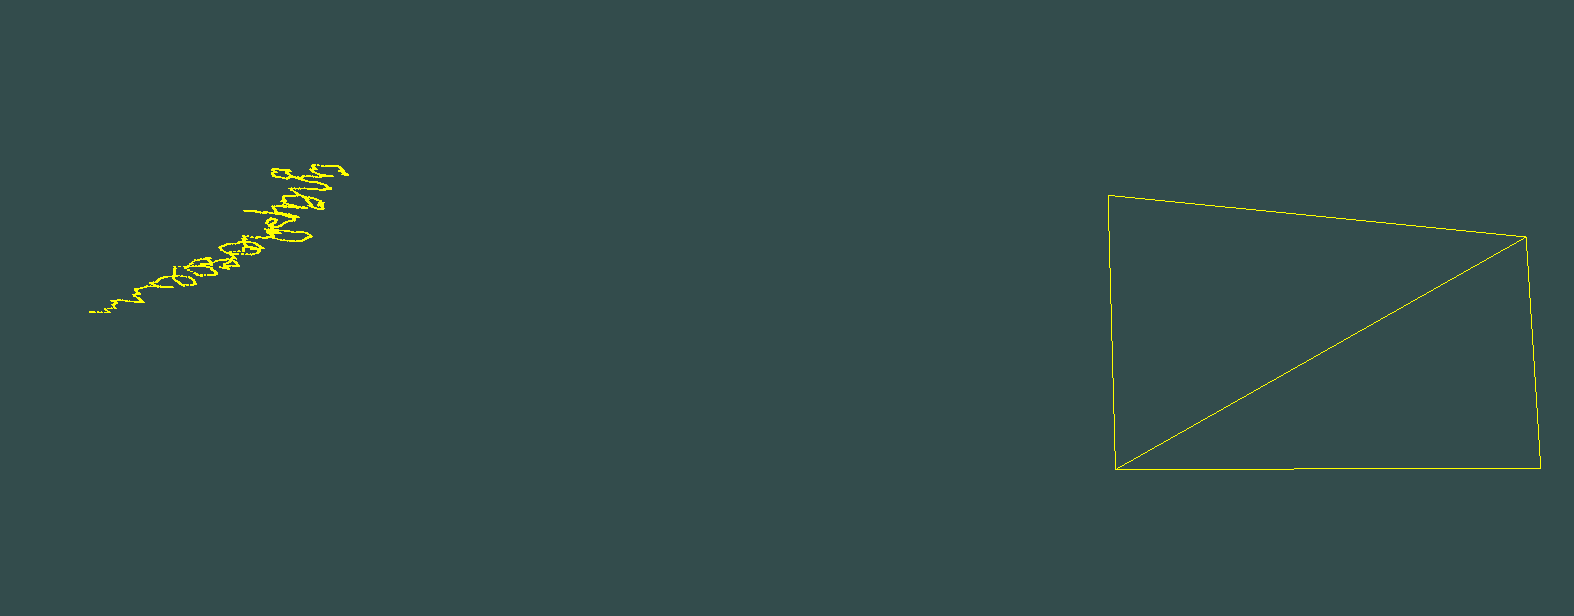
\includegraphics[width=\textwidth]{Modules/Picture/3d_2}
\caption{Image 3D - 2}
\label{3D2}
\end{figure}

\clearpage



\subsection{Langages et frameworks utilisés}

Le programme en lui-même est entièrement réalisé en C++, et différentes bibliothèques graphiques sont utilisées dans ce projet pour le traitement du flux vidéo, dans le but de faire du tracking sur le résultat, comme OpenGL et OpenCV. OpenGL est utilisé pour la reconstruction du mouvement de la plume en 3D, tandis qu'OpenCV est plus utilisé pour le traitement de l'image, notamment toutes les opérations faites dessus. De plus, Matlab est utilisé pour effectuer diverses opérations mathématiques sur les images, comme par exemple pour la calibration originelle servant à l'alignement pour la stéréo, ainsi que pour l'enlèvement de la distorsion. En effet, comme les caméras ont un grand angle, les éléments sur le bord de l'image sont courbés, il faut donc les remettre droits pour pouvoir travailler dessus.

\subsection{Fonctionnalités déjà implémentées}

Le programme tel qu'il nous a été fourni dispose de plusieurs fonctionnalités élémentaires permettant son bon fonctionnement. Parmi celles-ci, nous pouvons compter~:
\begin{itemize}
\item Le calibrage du dispositif dans sa globalité (caméras + surface d'écriture)
\item La synchronisation des deux caméras pour une reconstitution en trois dimensions des gestes lors de l'écriture
\end{itemize}
En plus de ces fonctionnalités, existe un dispositif matériel de capture. Ce dernier (Figure \ref{cameras}) est composé d'une structure en bois sur laquelle sont montées deux caméras. Ces dernières sont connectées à l'ordinateur par le biais d'un cable USB 3.0. Il est également possible de les bouger afin d'en ajuster les réglages.

\begin{figure}[!h]
\centering
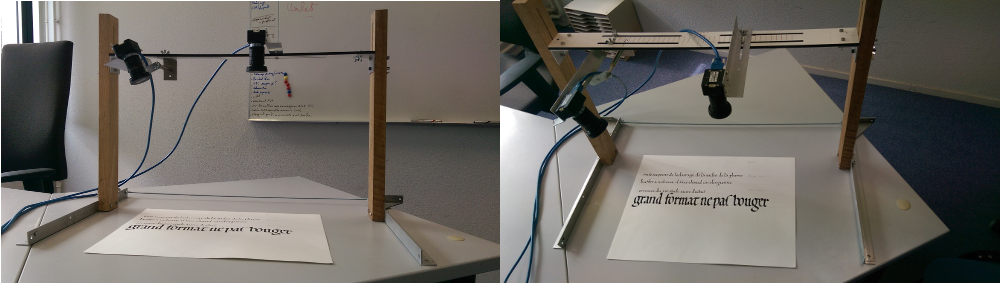
\includegraphics[width=\textwidth, height=4cm]{Modules/Picture/camerasPic.png}
\caption{Dispositif de capture stéréo}
\label{cameras}
\end{figure}

\subsection{Fréquence d'acquisition limitée}

Jusqu'alors, le programme ne possédait pas une fréquence d'acquisition suffisante de l'image. En effet, cette dernière n'était que de l'ordre de huit images par seconde. De ce fait, cette valeur ne permet pas une reconstituion précise en trois dimensions des gestes du calligraphe. L'objectif ici est donc de se rapprocher le plus possible de la fréquence maximale d'acquisition des caméras, soit trente images par seconde et ainsi gagner en précision lors du traitement.

\subsection{Impossibilité de bouger la feuille}

Avec la configuration actuelle, le calligraphe a l'impossibilité de bouger la feuille sur laquelle il écrit sous peine de perdre les réglages définis auparavant. Instinctivement, la personne qui écrit peut souhaiter bouger cette feuille et ainsi gagner en confort. Le but serait donc de trouver un moyen de gérer un changement de position de la feuille sans que cela n'affecte les résultats, en recalculant les réglages par exemple.

\subsection{Problèmes divers}

Initialement, l'éclairage du dispositif se faisait à l'aide de deux spots disposés de part et d'autre du calligraphe. Le problème majeur d'un tel moyen est la présence d'ombres à certains endroits rendant le traitement des images difficile, ainsi que la chaleur des lampes pouvant se réveler gênante à la longue. Un autre problème à gérer sont les gestes "inutiles" à l'acquisition que le calligraphe peut faire. En effet ce dernier peut par exemple vouloir étendre son bras pour se relaxer, geste qui sera pris en compte par le programme dans la reconstitution.

\section{Besoins fonctionnels et non fonctionnels}

	Une séparation des tâches était déjà effective dans le projet original, sur lequel travaillaient deux personnes : une personne travaillait sur l'acquisition stéréo, pendant que la seconde s'occupait de la modélisation 3D de la plume. Cette séparation a été conservée dans ce TER : \textsc{Gallet} Benoît et \textsc{Herrmann} Emmanuel s'occupent de la première partie, tandis que \textsc{Charpignon} Thibault et \textsc{Réty} Martin ont pris la deuxième.

\subsection{Augmentation de la cadence d'acquisition}

Naturellement, différentes idées nous sont venues pour augmenter la cadence d'acquisition de la vidéo en stéréo. Nous les détaillons ici, même si par la suite cette liste sera sûrement étoffée. Le programme fonctionne suivant plusieurs étapes~: Tout d'abord, une image est capturée à partir des deux caméras, puis les deux images sont encodées dans une vidéo. Une fois la capture finie, la vidéo est traitée afin de régler les problèmes de distorsion. Grâce à cette grande boucle qui capture les images deux par deux (une image par caméra), les vidéos finales commencent et terminent exactement au même moment, et permettent donc d'avoir simultanément la feuille d'écriture filmée sous deux angles différents. La modélisation en 3D sous OpenGL est alors possible. La seule variable est que plus la cadence d'acquisition est élevée, plus il y aura de FPS sur les vidéos finales, et plus la modélisation 3D de la plume sera précise. De plus, notre architecture et notre code doivent être assez robuste, pour que si un jour une troisième voire une quatrième caméra soient rajoutées, le nombre de FPS ne redescende pas drastiquement.

\subsubsection{Programmation parallèle}

Grâce à la programmation parallèle, qu'elle soit au niveau du CPU avec de l'OpenMP ou des threads, ou au niveau du GPU avec CUDA, nous pensons pouvoir accélérer l'acquisition des images, et donc des FPS sur les vidéos finales. Nous pensons regarder quelles parties peuvent être faites en parallèle, peut-être est-il possible d'uniquement récupérer une image tous les 3 centièmes de secondes (pour les 30 fps) dans le programme principal, et de faire tous les autres traitements dans des régions parallèles, avec par exemple un thread qui s'occupe d'ajouter la prochaine image à la vidéo, un autre thread qui enlève la distorsion de l'image, etc.

\subsubsection{Complexité}

Reprendre le code pour en examiner sa complexité est une autre piste envisagée pour augmenter les FPS. Nous pensons séparer cette idée en deux étapes~: Tout d'abord regarder la complexité de l'algorithme dans sa généralité, pour se rendre compte s'il y a problème ou non à ce niveau là, et voir les morceaux posant plus problème que le reste, puis faire des tests plus précisément sur ces parties pour voir ce qui ne va pas. Une analyse légerement différente pourra être effectuée, avec des tests fontionnels calculant quelle partie prend le plus de temps. Ces tests sont très complémentaires de ceux de complexité, à eux deux ils devraient mettre en exergue les problèmes principaux du code actuel.

\subsubsection{Modularité}

Outre cette analyse de la complexité, une mise au propre du code devra être effectuée. En effet, tout se trouve dans la fonction \texttt{main}, dans deux grandes boucles. Une partie de notre travail sera donc de modulariser cette fonction, de la séparer en plusieurs méthodes afin de gagner en clarté. De plus, l'ajout de l'option \texttt{-O2} lors de la compilation permet d'optimiser sensiblement les performances. Nous prévoyons par la suite d'utiliser à la place \texttt{-O3} qui compilera les fonctions sur une seule ligne, ce qui permettra de minimiser le coût de cette modularisation du code lors de son exécution.

\subsubsection{Généralisation}

Sinon, le dernier axe sur lequel travailler sera la généralisation du nombre de caméras. Pour l'instant, tout dans le code est fait pour deux caméras, avec du code dupliqué pour chaque action. La généralisation pour \textit{n} caméras sera facilitée par la modularisation du code, et permettra par la suite de rajouter une ou plusieurs caméras sans modification majeure, uniquement en changeant quelques \texttt{\#define}.


\subsection{Tracking de la plume}

Comme pour la partie sur l'augmentation de la cadence d'acquisition, différents problèmes sont à résoudre pour le tracking. Cette partie permet de traiter les vidéos produites par les caméras et d'en ressortir une trace des mouvements effectués par le calligraphe. L'étudiant de Polytech qui a travaillé sur cette partie a recherché différents algorithmes permettant d'effectuer ce tracking. Son étude se focalise sur deux algorithmes basés sur l'apprentissage de toutes les apparences observées de l'objet et d'une estimation des erreurs pour ensuite les éviter:

\begin{itemize}

\item Tracking Learning Detection (TLD)

\item Kernelized Correlation Filters (KCF)

\end{itemize}

  
\subsubsection{Analyse de la complexité}

Heureusement, l'analyse des deux algorithmes a déjà été faite par l'étudiant, ce qui a montré que dans notre cas l'algorithme KCF est le plus efficace. Son étude est basée sur plusieurs critères, la déviation moyenne des deux vidéos, le nombre de frames et le temps de calcul. Seul le premier critère est réellement différent entre les deux méthodes. C'est cette différence qui a orienté son choix vers l'algortihme KCF. \\

Ici, notre premier axe de recherche sera orienté vers une étude complémentaire de ces algorithmes pour vérifier la véracité de l'analyse précédente. Pour cela nous allons réutiliser les critères d'études et ensuite essayer d'en trouver d'autres pour confirmer le choix. Dans un second temps il nous faudra rechercher d'autres algorithmes ou méthodes de programmation pour améliorer le tracking.

\subsubsection{Gestion mouvements}

Bien entendu, le choix des algorithmes n'est pas la seule difficulté, nous faisons face également à des contraintes physiques liées aux mouvements du calligraphe. Par exemple il doit prendre des temps de repos afin de garder sa fluidité d'écriture en faisant des gestes de relaxation du poignet. Ces mouvements ne doivent pas être pris en compte par l'algorithme de tracking afin d'éviter des erreurs sur la représentation du mouvement. \\

Résoudre ce problème ce problème pourrait passer par la sauvegarde à un temps T et à un temps T+1 d'une image de la partie suivie. Puis analyser la différence entre les deux images et en ressortir un résultat positif ou négatif. Cela reviens à prendre la dernière image où le calligraphe écrit et une autre image qui permettra de voir si le mouvement est la continuité de l'écriture ou un mouvement parasite.

\subsection{Autres axes de travail}

\subsubsection{Zone de capture}

En écrivant, le calligraphe doit de temps en temps bouger la feuille pour se repositionner et continuer sa rédaction. L'algorithme actuel ne gère pas ce mouvement, ce qui nécessitait après chaque mouvement de la feuille un nouveau calibrage des caméras et de la zone de capture. Une solution possible pour résoudre ce problème est la mise en place d'un système de cadre pour que le calligraphe sache la zone dans laquelle il peut écrire. Ce cadre pourrait être un marquage sur la feuille qui délimitera la zone de capture. Nous souhaitons également rechercher d'autre solutions possibles pour résoudre ce problème.

\subsubsection{Changement de la structure}

Pour le moment le dispositif de capture ne comporte que deux caméras et des angles de prises de vue bien définis. L'ajout d'une caméra et le repositionnement des deux premières peut permettre de rendre plus précise l'acquisition. De cette manière nous aurions à notre disposition des informations supplémentaires pour améliorer la reconstruction du mouvement. Il nous faut donc tester différentes configurations et choisir la meilleure \\

Un des facteurs majeurs de la capture d'image est la lumière. En effet, il est important que la feuille soit bien éclairée pour le confort et l'écriture du calligraphe. La structure actuelle ne comporte pas d'éclairage du tout, il était nécessaire d'avoir une lampe d’appoint. Une solution simple est l'ajout d'une plaque LED pour avoir une luminosité uniforme sur toute la feuille. \\

Tous ces changements devront peut-être être accompagnés d'une refonte totale du dispositif.

\subsubsection{Compatibilité Windows - Linux - MacOS}

A l'origine, les étudiants ont développé tout le code sur Windows et plus particulièrement sur l'IDE Visual Studio (C++). Pour rendre le code réutilisable à l'avenir nous avons comme objectif de pouvoir l'utiliser sur tous les systèmes d'exploitation (Linux/MacOS en plus). Pour cela il est nécessaire d'uniformiser le code et de se servir de librairies communes pour standardiser au mieux le projet.

\section{Prototypes et résultats de tests préparatoires}

Il nous fallait, pour bien prendre en main le projet, tester réellement le dispositif de lancement du logiciel jusqu'à la capture vidéo. Nous avons dû  procéder à l'installation de tout l'environnement de travail nécessaire (FlyCap2, OpenCV, OpenGL) et l’acquisition des premières vidéos avec les caméras mises à notre disposition. \\

Notre première tâche a été de transférer le code initial sous Linux et ainsi le tester directement. Les tests ont été concluants et le premier groupe a pu commencer directement à améliorer le système. Le second, quant à lui, a récupéré le code concernant le tracking mais a rencontré de gros problèmes lors de son passage de Windows vers Linux.
Le code n'utilisant pas des fonctions standards, important des librairies en "dur" et étant peu commenté, il est pour le moment impossible de tester le code de l'étudiant qui travaillait sur le tracking l'année précédente. Pour y remédier le second groupe a dû repasser cette partie du projet sur Windows le temps de bien comprendre les différents problèmes et de les corriger.

\section{Planning}

Les petites barres sur le diagramme de Gantt (Figure \ref{gantt1}) correspondent aux différentes réunions que l'on a eu, suivies des noms des participants. Les plus grandes correspondent quant à elles aux tâches effectuées. Il y en a peu pour le moment car la phase de compréhension et d'installation des composants a été relativement longue.

\begin{figure}[!h]
\centering
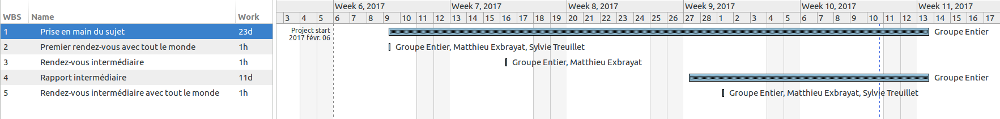
\includegraphics[width=\textwidth, height=3cm]{Modules/Picture/diag1.png}
\caption{Diagramme de Gantt de la première partie}
\label{gantt1}
\end{figure}

\newpage


\bibliographystyle{plain}
\nocite{*}
\bibliography{Modules/biblio}
 
 
\end{document}

\grid
